\documentclass[a4paper]{article}

%% Language and font encodings
\usepackage[francais]{babel}
\usepackage[utf8x]{inputenc}
\usepackage[T1]{fontenc}

%% Sets page size and margins
\usepackage[a4paper,top=3cm,bottom=2cm,left=3cm,right=3cm,marginparwidth=1.75cm]{geometry}

%% Useful packages
\usepackage{amsmath}
\usepackage{graphicx}
\usepackage[colorinlistoftodos]{todonotes}
\usepackage[colorlinks=true, allcolors=blue]{hyperref}


\title{Détection de la trajectoire d'une balle de tennis}
\author{Raphaël Montaud et Cyril Malbranke}

\begin{document}
\maketitle

\begin{abstract}
	L'objectif est de pouvoir arbitrer un match de tennis en annonçant les balles qui rebondissent en dehors du terrain. Dans un premier temps nous travaillerons avec une caméra classique (donc une seule image de la même scène) et nous nous pencherons ensuite sur le même problème avec une caméra 3D (donc deux images différentes de la même scène).
\end{abstract}


\section{Benchmarking et choix des données de travail:}

\subsection{La technologie Hawk-Eye}
L'état de l'art est déjà bien développé pour ce qui est du suivi de la trajectoire d'une balle. En effet, la technologie Hawk-Eye opère déjà dans plusieurs sports et peut remplacer les décisions de l'arbitre dans certaines compétitions officielles. Par exemple au tennis, dans certains tournois comme le Qatar Total Open, les joueurs peuvent contester la décision de l'arbitre à trois reprises au cours d'un set en faisant appel à la technologie Hawk-Eye.
Le suivi de la trajectoire se fait avec l'aide de 6 caméras haute performance qui traquent la balle. Une triangulation permet ensuite de connaître la position de la balle en trois dimensions. Enfin, le nuage de points obtenus est transformé en une courbe 3D qui correspond à la trajectoire la plus probable.

\subsection{Choix des données}
Il est difficile de trouver des images de matchs de tennis de qualité suffisante. En effet, même une très bonne qualité d'image comme la 4k ne suffit pas à traquer la position de la balle. Si il n'y pas assez d'images par secondes, la balle peut apparaître très floue sur les images ce qui rend la tâche très compliquée. Nous avons donc contacté l'entreprise Hawk-Eye Innovations pour être en mesure de tester nos algorithmes sur des données réelles. Cependant, l'issue de cette démarche étant incertaine, nous avons cherché une autre source de données.

Notre choix s'est finalement porté sur des images de jeux vidéos de tennis. Celles-ci sont effectivement de très bonne qualité, et il n'y a pas de flou autour de la balle lorsque l'on fait un arrêt sur image. Cela simule donc des images haute fréquence et de bonnes qualité. De plus, les images varient peu (notamment en termes de lumière), ce qui permet de simplifier le problème dans un premier temps. En revanche, la caméra bouge contrairement aux images des caméras Hawk-Eye et cela va donc nous obliger à procéder à un prétraitement.

\section{Preprocessing}
\subsection{NOM DU LOGICIEL}
Il faut dans un premier temps transformer la vidéo en une séquence d'images. Pour cela nous avons utilisé le logiciel NOM DU LOGICIEL. Le format d'une vidéo est en fait très compressé et quelques minutes de vidéo (donc quelques Mo) ont produit plus d'un Go d'images.

\subsection{Stabilisation de l'image}
Dans le cadre de notre premier travail avec une seule image, il est nécessaire de stabiliser l'image. L'objectif est ici que les lignes du terrains aient toujours la même position dans l'image. Ainsi, cela facilite grandement le travail d'analyse de la trajectoire. Pour cela nous avons choisi une image de référence. Puis, nous calculons l'homographie qui permet de passer d'une image à l'image de référence. Pour cela, il existe plusieurs façons de faire. On peut par exemple citer les méthodes de corrélation d'images avec les points de Harris. Pour notre part, nous avons décidé de prendre avantage de la spécificité du problème. Nous faisons de la détection de lignes qui nous permet de trouver les quatre coins du terrains et ainsi calculer l'homographie qui relie l'image à celle de référence.

Pour la détection de lignes, nous utilisons d'abord un filtre de Canny qui permet de faire de la détection de contours. Puis nous appliquons l'algorithme Hough Lines de OpenCv. Cet algorithme repose sur un principe assez simple mais il fournit des résultats satisfaisants. Pour chaque droite possible (rho, theta), on regarde combien de points appartiennent à cette ligne (nous rappelons ici que l'image est binaire à la sortie du filtre de Canny). Les droites avec le plus de votes sont retenues. Nous identifions ensuite les lignes qui nous intéressent grâce à de simples conditions sur la position et l'orientation. Cependant, le fait que la caméra bouge rend ce conditionnement difficile. Il faut garder des conditions larges, ce qui fait que certaines images renvoient des lignes avec des positions abhérentes. Il est donc important d'appliquer une méthode d'élimination de valeurs abhérentes.


Pour cela nous appliquons plusieurs filtres sur les données:
Un premier filtre consiste à calculer l'écart au carré de l'homographie par rapport à l'homographie moyenne. Cela permet d'avoir un tracé qui correspond aux mouvement de caméras, comme on peut le voir dans la figure 1. Les mouvements de caméras extrêmes correspondent à des valeurs autour de 25 000. Toutes les valeurs au dessus de ce seuil sont donc considérées comme abhérentes et l'homographie calculée est remplacée par l'homographie de l'image précedente.

\begin{figure}[h!]
\centering
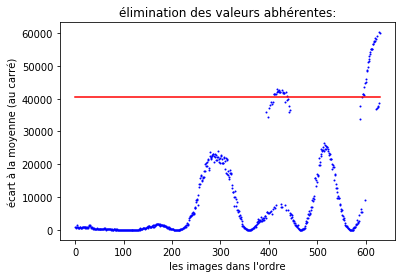
\includegraphics[width=\textwidth]{valeurs_abherentes.png}
\end{figure}

Ensuite, la variation des homographies est censée être continue. Nous éliminons donc les homographies où la variation est jugée trop rapide. Il est d'ailleurs assez facile d'identifier graphiquement les points aux valeurs abhérentes.

\begin{figure}[h!]
\centering
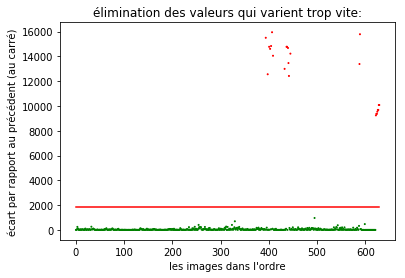
\includegraphics[width=\textwidth]{valeurs_abherentes_2.png}
\end{figure}

Enfin nous appliquons un filtre gaussien sur les homographies calculées pour obtenir un résultat plus lisse.

Le résultat obtenu est très satisfaisant. Cependant, beaucoup d'améliorations sont envisageables pour cette partie du projet. Il y a d'abord un certain nombre de paramètres à optimiser. Ensuite les lignes du terrains sont considérées comme si elles n'avaient pas d'épaisseur, or, pour obtenir des résultats plus précis, il faudrait chercher à distinguer le bord extérieur et le bord intérieur. Nous avons décidé de ne pas nous attarder plus que ça sur cette partie car c'est un 'faux problème' étant donné qu'il n'y a pas de raisons de s'imposer des caméras qui bougent, et le résultat sur la séquence d'images obtenu est suffisant pour pouvoir poursuivre nos recherches.

\section{Détection d'objets}


\section{Travail en 3D:}



\section{Conclusion}
Après nous être fixés un système probabiliste pour les rencontres sportives, nous avons pu modéliser le déroulement d'un championnat de football. Comme nous l'avons montré, la simulation de Monte-Carlo standard ne suffit pas pour étudier des événements rares sans l'aide de super-ordinateurs. Le recours à la méthode de décalage en probabilité permet d'obtenir des estimations de probabilités pour les événements rares. Ensuite, nous nous sommes penchés sur le comportement de différentes distributions de forces des équipes dans le cas ou le nombre de joueur tend vers l'infini. La théorie montre que certaines distributions sont plus propices à la défaite du meilleur joueur, mais l'expérience montre que certains de ces comportements ne sont sensibles que pour un très grand nombre de joueurs, ce qui nous éloigne du sujet des championnats de football, mais qui peut être valide dans d'autres domaines d'application du modèle de Bradley-Terry comme la comparaison de revues scientifiques. Enfin nous avons montré que les enjeux économiques dans les résultats de football sont importants et nous avons proposé une méthode pour en tirer profit. Après nous être fixé notre modèle probabiliste, nous optimisons nos paramètres pour nous rapprocher de la réalité. Nous pouvons alors utiliser ces paramètres pour estimer des événements rares grâce aux méthodes vues précédemment.


\section{Bibliographie}
R. Chetrite, R. Diel, M. Lerasle \textit{The number of potential winners in Bradley-Terry model in random environment}, Ann. Appl. Probab., 2016. https://arxiv.org/abs/1509.07265 \\

S. Escalón. \textit{Le ballon rond à l’épreuve des probabilités}, Le Journal du CNRS, 2017. https://lejournal.cnrs.fr/articles/
le-ballon-rond-a-lepreuve-des-probabilites.
\end{document}
